\chapter{Estado del Arte}

\section{Codificación por Octree}

La codificación por octree es una técnica jerárquica para representar objetos espaciales que aprovecha la coherencia espacial presente en la mayoría de las nubes de puntos y objetos tridimensionales \cite{meagher1982geometric,loop2016microsoft}. Esta técnica organiza la información en una estructura arbórea en la que cada nodo representa un cubo disjunto en el espacio, cuyo tamaño decrece exponencialmente a medida que se desciende por los niveles del árbol. De esta forma, cada nodo corresponde a una región del universo y se le asigna una propiedad que describe dicha región.\\

Si un nodo describe completamente su región —por ejemplo, si el cubo está completamente vacío o completamente ocupado— se considera un nodo terminal o hoja. En caso contrario, existe una ambigüedad que se resuelve dividiendo la región en ocho subregiones o octantes, que corresponden a los nodos hijos del nodo padre. Esta subdivisión recursiva permite representar objetos con un grado de detalle variable, adaptando la precisión espacial a la complejidad local de la nube de puntos \cite{meagher1982geometric}.\\

\begin{figure}
    \centering
    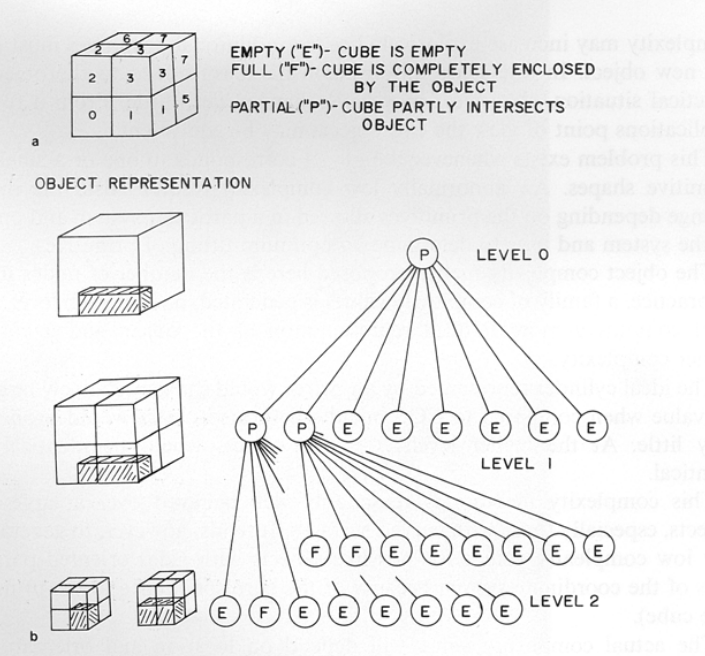
\includegraphics[width=0.5\linewidth]{img/estado_del_arte/octree.png}
    \caption{Representación simple del formato de la codificación por Octree}
    \label{fig:octree}
\end{figure}

Una ventaja esencial de esta estructura es que utiliza una única forma primitiva, el cubo, lo que simplifica tanto el almacenamiento como las operaciones sobre los datos. Además, al representar el objeto a múltiples niveles de resolución, el octree permite gestionar la memoria de manera eficiente, almacenando los detalles más finos sólo cuando es necesario y manteniendo un nivel más grueso cuando el detalle no es crítico. Esto facilita también realizar operaciones espaciales como la detección de colisiones, la visualización con ocultación y operaciones booleanas de forma eficiente, ya que el recorrido jerárquico permite acceder a las regiones del espacio de manera ordenada, evitando búsquedas exhaustivas \cite{meagher1982geometric}.\\

Asimismo, la estructura jerárquica del octree permite que muchas operaciones puedan ser detenidas en niveles superiores cuando la precisión requerida se ha alcanzado, lo que reduce significativamente el costo computacional. Por otro lado, la naturaleza dividida del árbol, donde cada nodo genera hasta ocho subcálculos independientes, hace que el procesamiento pueda ser paralelizado fácilmente, mejorando la velocidad en sistemas con múltiples procesadores.\\

En cuanto a la representación, cada nodo en el octree está identificado por una dirección única que indica su posición espacial relativa al nodo raíz y su nivel dentro de la jerarquía. Las propiedades asignadas a los nodos pueden ir desde una simple clasificación en estados como vacío, parcialmente lleno o completamente lleno, hasta incluir atributos complejos como tipo de material, color o densidad, ampliando así la riqueza de la representación \cite{loop2016microsoft}.\\

Aunque la codificación por octree puede requerir un mayor consumo de memoria, generalmente proporcional al área superficial del objeto representado, su capacidad para modelar la estructura espacial de la nube de puntos de manera compacta y adaptativa la convierte en una herramienta esencial para la compresión y manipulación eficiente de datos tridimensionales \cite{meagher1982geometric}. Así, el codificado por octree abre la posibilidad de aprovechar la correlación espacial inherente a las nubes de puntos, permitiendo una representación estructuralmente coherente y eficiente que facilita tanto el almacenamiento como el procesamiento posterior \cite{loop2016microsoft}.

\section{Run Length Golomb-Rice Entropy Coder}\label{sec: rlgr}

El codificador de entropía Run Length Golomb-Rice (RL-GR) es un método efectivo y de baja complejidad para la compresión sin pérdida de secuencias binarias con estructuras de tipo \textit{run-length}, es decir, secuencias con repeticiones consecutivas del mismo símbolo \cite{malvar2006adaptive,sayood2006introduction}. Combinando codificación por longitud de carrera (Run Length) con codificación Golomb-Rice, este método permite representar eficientemente tanto secuencias de ceros prolongadas como valores pequeños comunes en señales residuales.

La codificación Golomb-Rice es un caso particular de codificación de Golomb donde el parámetro divisor es una potencia de dos, lo que permite una implementación computacionalmente eficiente \cite{malvar2006adaptive}. Este codificador es ampliamente utilizado en estándares de compresión como MPEG y JPEG-LS \cite{jpeg1992}, debido a su equilibrio entre rendimiento y simplicidad. En el contexto de nubes de puntos, RL-GR se emplea para comprimir mapas de ocupación, residuos de predicción o secuencias binarias derivadas del escaneo espacial jerárquico, donde los datos presentan redundancia local y patrones repetitivos.

\section{\textit{Learning separable transforms by inverse covariance estimation}} \label{sec: lst_ice}

Este trabajo presenta un enfoque para diseñar transformadas adaptativas que se ajusten automáticamente a las características específicas de los datos de entrada. La idea principal es que en lugar de usar transformadas fijas como DCT o DST, se pueden crear transformadas que cambien según las propiedades estadísticas de la señal a procesar.\\

El aporte más relevante son las Transformadas Trigonométricas Discretas Paramétricas (p-DTTs), que se basan en la representación de la señal como un grafo de línea. Un grafo de línea es simplemente una cadena de nodos conectados secuencialmente, donde cada nodo representa un píxel o muestra de la señal. La innovación clave consiste en agregar conexiones adicionales llamadas \textit{self-loops} en los extremos de esta cadena, lo que modifica las propiedades de la transformada resultante.\\

Matemáticamente, las p-DTTs se definen mediante dos parámetros $(\alpha, \beta)$ que controlan el peso de estos \textit{self-loops} en el primer y último nodo del grafo respectivamente. Cuando $\alpha = \beta = 0$, se obtiene la transformada DCT-2 clásica. Variando estos parámetros se pueden generar otras transformadas conocidas como DST-4 o DST-7, pero también crear nuevas transformadas adaptadas a características específicas del contenido modificando el laplaciano.\\

\begin{equation}
    L(\alpha, \beta) = \text{diag}(\alpha, 0, \ldots, 0, \beta) + L_{DCT}
= \begin{bmatrix}
\alpha & 0 & \cdots & 0 & 0 \\
0 & 0 & \cdots & 0 & 0 \\
\vdots & \vdots & \ddots & \vdots & \vdots \\
0 & 0 & \cdots & 0 & 0 \\
0 & 0 & \cdots & 0 & \beta
\end{bmatrix} + \begin{bmatrix}
1 & -1 & 0 & \cdots & 0 \\
-1 & 2 & -1 & \cdots & 0 \\
0 & -1 & 2 & \cdots & 0 \\
\vdots & \vdots & \ddots & \ddots & \vdots \\
0 & 0 & \cdots & -1 & 1
\end{bmatrix}
\end{equation}


Ocupando esta metodología se pueden replicar un conjunto preciso de transformadas paramétricas demostrando la capacidad de adaptar dinámicamente las transformadas gráficas. Aplicando distintos valores, se pueden obtener según la dinámica de la señal a procesar un conjunto de señales, según la siguiente tabla:

\begin{table}[H]
    \centering
    \caption{Relación entre parámetros $\alpha$ y $\beta$ con las transformadas seleccionadas}
    \begin{tabular}{c|ccc}
    \toprule
    $\alpha \backslash \beta$ & 0 & 1 & 2 \\
    \midrule
    0 & DCT-2 & DCT-8 & DCT-4 \\
    1 & DST-7 & DST-1 & DST-5 \\
    2 & DST-4 & DST-6 & DST-2 \\
    \bottomrule
    \end{tabular}
\end{table}

La relevancia de este enfoque para nubes de puntos radica en que demuestra cómo la modificación estructural de un grafo mediante \textit{self-loops} puede mejorar significativamente el rendimiento de las transformadas. Mientras que las p-DTTs operan sobre grafos de línea simples para señales 2D, el principio subyacente de adaptar la estructura del grafo según las características locales de la señal puede extenderse a grafos 3D más complejos para el procesamiento de atributos de color en nubes de puntos.

\section{\textit{Point Cloud Attribute Compression With Graph Transform}}\label{sec: pcac_geometric}

La compresión de atributos de nubes de puntos mediante transformada de grafos es una técnica avanzada que explota la estructura irregular de los datos tridimensionales \cite{zhang2014point,pavez2020region}. A diferencia de los métodos clásicos que utilizan DCT o \textit{wavelets}, la transformada de grafos permite modelar relaciones entre puntos a través de un grafo, donde los nodos representan puntos y las aristas modelan su proximidad o conectividad.\\

La transformada de Fourier sobre grafos (GFT) permite descomponer los atributos, como el color o la reflectancia, en una base adaptada a la estructura del grafo, capturando mejor la correlación espacial entre puntos \cite{ortega2022gsp}. De esta forma, la energía de los atributos tiende a concentrarse en unos pocos coeficientes de baja frecuencia, lo que permite una compresión más efectiva.\\

Considerando que la información geométrica ya ha sido codificada mediante métodos como los mencionados anteriormente en la sección de codificación por octree, se asume que la información estructural ya la posee el decodificador y por tanto la compresión de los atributos puede utilizar esta información sin necesitar agregar instrucciones mayores respecto a la información estructural \cite{loop2016microsoft}.\\

Luego, este método construye un grafo basándose en distancias discretas de puntos voxelizados donde las conexiones existirán siempre que dicha distancia no supere cierto umbral. Estos pesos o valores de arista son inversamente proporcionales y tienen la diagonal cúbica como límite describiéndose de la siguiente manera:

\begin{equation}
    w_1 = 1, \quad w_2 = \frac{1}{\sqrt{2}}, \quad w_3 = \frac{1}{\sqrt{3}}
\end{equation}

Lo que describirá una matriz de adyacencia simétrica de la forma:
\[
A = 
\begin{bmatrix}
0   & w_3 & w_2 & 0   & 0   & 0 \\
w_3 & 0   & w_1 & w_3 & 0   & 0 \\
w_2 & w_1 & 0   & w_2 & 0   & 0 \\
0   & w_3 & w_2 & 0   & w_1 & w_2 \\
0   & 0   & 0   & w_1 & 0   & w_1 \\
0   & 0   & 0   & w_2 & w_1 & 0
\end{bmatrix}
\tag{5}
\]

Ocupando esta construcción de grafo, se procede a hacer el proceso de transformada gráfica descrita en el marco teórico \cite{ortega2022gsp}. Este entregará un laplaciano que se asegura es una matriz semidefinida positiva. Luego, entendiendo que la transformada gráfica contiene solo información disponible en el decodificador, el mensaje se convierte en la codificación de los coeficientes de las bases posterior a su cuantificación.\\

Al ser este un enfoque nuevo para su época, la comparación se hace respecto a la DCT de una dimensión para el encadenamiento de todos los bloques. Sean el nivel 5 bloques de 16x16x16, el nivel 6 bloques de 8x8x8, el nivel 7 bloques de 4x4x4 y el nivel 8 bloques de 2x2x2, se muestran los siguientes resultados en la siguiente figura:

\begin{figure}
    \centering
    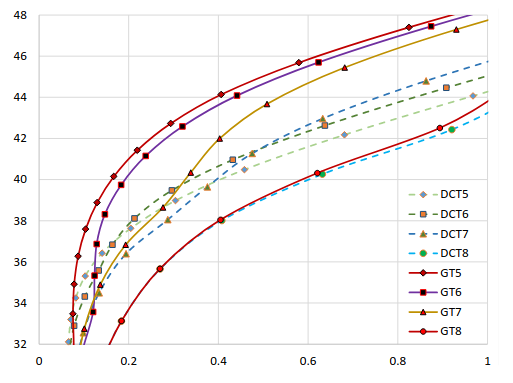
\includegraphics[width=0.5\linewidth]{img/estado_del_arte/block_GFT.png}
    \caption{Rendimiento de compresión (en dB) frente a la tasa de bits (en bpv) para el codificador propuesto utilizando una Transformada de Grafos y DCT para los niveles de octree 5, 6, 7 y 8 (correspondientes a tamaños de cubo de 16, 8, 4 y 2, respectivamente) \cite{zhang2014point}}
    \label{fig:block_gft}
\end{figure}

Los datos utilizados provienen de nubes de puntos 3D generadas en tiempo real
